\documentclass{book}

\usepackage{makeidx, cite, indentfirst}
\usepackage{amsmath, amssymb, amsfonts, graphicx}
\usepackage[english, greek]{babel}
\usepackage[margin=1in]{geometry} 

\makeindex

\begin{document}
\selectlanguage{english} 

\frontmatter

\begin{titlepage}
    \centering
    % Insert the figure on the title page
    
\includegraphics[width=0.5\textwidth]{figures/icl_logo.jpeg} 
    \vfill
    {\Huge\bfseries Introduction to probability theory and statistical inference\par}
    \vspace{1cm}
    {\Large Jes\'us Urtasun Elizari\par}
    \vspace{1cm}
     {\Large Research Computing and Data Science\par}
    \vspace{1cm}
    {\large\today\par}
    \vspace*{\fill}
\end{titlepage}

\selectlanguage{english}
\tableofcontents

\chapter*{Index}
\addcontentsline{toc}{chapter}{Index}
\clearpage
\printindex

\mainmatter


% Chapter - Introduction
\chapter{Introduction}

In the following pages one will find an introductory course to the theory of probability and statistical inference, aiming to cover both foundations and basic mathematical concepts, but also practical tools to deal with real data science problems, such as bayesian inference and hypothesis testing. The text is composed by six chapters, together with some appendix reviewing basic mathematical concepts, and a bibliographic note. The purpose of these lecture notes is to make both probability and statistical analysis an easy, engaging and exciting topic for anyone interested, without the need for prior experience or deep mathematical training.\\

First, we will introduce the idea of probability and random events with simple and intuitive examples, and we will see how different approaches have been used to model information and chance. Then we will discuss a series of mathematical ways to formally define random processes, also referred to as \textit{stochastic}. We will introduce the idea of \textit{distribution}, uncertainty and variability, and we will learn how to build quantities - we will call them \textit{estimators}, or \textit{expected values} - that represent the information we have about such random measurements. 

In the second part we will address the difference between prediction and inference, and discuss a set of subjects normally grouped under the name of \textit{hypothesis testing}. Here we will introduce how to quantify certainty and bias, how to model significance and the idea of hypothesis tests. Finally, we will briefly discuss more modern topics, such as bayesian statistics, and further stochasticity with the so-called Markov processes.\\

Ideas such as stochasticity and randomness have deep historical roots. Ancient civilizations, from Babylonians, Egyptians, and Greeks, faced uncertainty in games of chance, commerce, and divination, among others. The oldest known dice date back over 5,000 years, indicating an early human fascination with randomness. While these cultures did not develop formal mathematical probability, they recognized patterns in random events and attempted to predict outcomes based on empirical observations and superstitions.\\
\indent Greek philosophers such as Democritus and Aristotle debated the nature of chance and determinism [...]. The Roman philosopher Cicero distinguished between chance events and those governed by fate, foreshadowing later discussions on probability. It would not be until medieval times, where mathematicians like Gerolamo Cardano (1501–1576) made early contributions by analyzing gambling problems and laying the groundwork for probability theory.\\

Such intuitions properly formalized probability as a mathematical discipline in the 17th century, with the correspondence between Blaise Pascal and Pierre de Fermat, who devised combinatorial methods to solve problems related to games of chance. Their work introduced fundamental ideas such as expected value and laid the foundation for later advances by Christiaan Huygens, Jacob Bernoulli, and Abraham de Moivre. Bernoulli’s \textit{Ars Conjectandi} (1713) introduced the Law of Large Numbers, establishing that observed frequencies converge to theoretical probabilities over many trials. All these names and topics will be covered in detail through chapters 2 and 3.\\

At the end of each chapter there will be a series of exercises and coding examples to illustrate and demonstrate the concepts discussed. To avoid misconceptions, let us emphasize here that both, probability and statistics are branches of mathematics that aim to quantify uncertainty, chance and information in the random events, \textit{much earlier} than computers, coding languages, Python, R or P-values were even conceived. The data-oriented, practical ways in which we nowadays focus probability and stats, heavily relying on computation, is just a consequence of the fact that automatized measurements are nowadays available and trendy in modern times.

As one could guess already, a proper understanding of such topics - uncertainty, variation, probability, chance - can be applied to describing a vas amount of real-world phenomena, ranging from gambling and statistical inference, to data analysis in physics, biology, machine learning and quantum mechanics. In the same way we learn to count and measure, we could try to assign numerical values to the likelihood of different outcomes in an experiment, or quantify the level of certainty - or \textit{surprise} - for such unknown result. The modern approach to probability and its fundamental concepts are summarized in the axioms established by the Russian mathematician Andrey Kolmogorov, in the early 1930s. Some people may find surprising that such an old topic was not properly formalized until such recent times. We will cover this with a bit more detail in Chapter 1.\\

This is intended to be a complete introductory course, and no previous mathematical background is required. By keeping the theory simple and always followed by examples, we will build the definitions and quantities from simple to more complex. All mathematical formulas will be introduced with rigorous notation, but keeping in mind that is not the symbols or the numbers, but the intuitions and the general understanding, what we are behind.

Let's start defining a couple of quantities most people are already familiar with, and for which they may have some intuition, as a warmup example. Let's illustrate with an example how to properly define the \textit{mean} and \textit{variance} of a set of observations.\\
	
Imagine we are doing an experiment and we measure some variable - let's call it $x$ - that can be anything (position at a given time, energy of some system, concentration, ...). We repeat the measurement three times and we get first 1, then 2, and the last time 3. That will be our set of observations, or our \textit{sample}, $x_{1}$. We could write it as a list, or a \textit{vector} - in the following way as

\begin{equation}
x_{1} = \{1, 2, 3\} \nonumber. 
\end{equation}

Keep in mind that from the mathematics perspective the word \textit{vector} has a different meaning, with subtleties related to algebraic operations and relations they should satisfy, but for the purpose of this course, where we prioritize above all simplicity, a vector and a list of numbers will be essentially the same thing.\\

We define the \textit{mean} - or \textit{average} - $\bar{x}$ of an arbitrary large sample of $N$ observations, as the sum of all elements divided by the total.

\begin{equation}
\bar{x} = \frac{1}{N} (x_{1} + x_{2} + ... + x_{N}) = \frac{1}{N} \sum_{i = 1}^{N} x_{i}
\end{equation}

Here we denote the sum of all elements with the greek letter $\sum$, starting with the first one ($i = 1$) and until the last one ($i = N$). If we now substitute that expression for our set $x_{1}$, which has just $N = 3$ observations, we get

\begin{equation}
\bar{x}_{1} = \frac{1}{3} \sum_{i = 1}^{3} x_{i} = \frac{1}{3} (1 + 2 + 3) = 2 \nonumber
\end{equation}

As we see, the mean is just a quantity that captures some information about the "central" value, where the bulk of event are. In a similar way, we can define the \textit{variance} as a quantity that captures how far are the elements of the sample from the mean value.

\begin{equation}
s^{2} = \frac{1}{N - 1} \sum_{i = 1}^{N} (x_{i} - \bar{x})^{2}. 
\end{equation}

Again, just by substituting that expression for our set $x_{1}$, which has just $N = 3$ observations, we get

\begin{equation}
s_{1}^{2} = \frac{1}{3 - 1} \sum_{i = 1}^{3} (x_{i} - \bar{x})^{2} = \frac{1}{2} \big((1 - 2)^{2} + (2 - 2)^{2} + (2 - 3)^{2}\big) = \frac{1}{2} (1 + 0 + 1) = 1 \nonumber
\end{equation}

which we could interpret as, on average, the elements of the list being \textit{one unit} away from the mean.

As an exercise, try to compute both the mean and variance for a second sample, let's say

\begin{equation}
x_{2} = \{4, 5, 6\} \nonumber. 
\end{equation}

You should get: 

\begin{equation}
\bar{x}_{2} = \frac{1}{3} \sum_{i = 1}^{3} x_{i} = \frac{1}{3} (4 + 5 + 6) = 5 \nonumber
\end{equation}

\begin{equation}
s^{2}_{2} = \frac{1}{3 - 1} \sum_{i = 1}^{3} (x_{i} - \bar{x})^{2} = \frac{1}{2} \big((4 - 5)^{2} + (5 - 5)^{2} + (6 - 5)^{2}\big) = \frac{1}{2} (1 + 0 + 1) = 1 \nonumber
\end{equation}

Again, our mean $\bar{x}_{2} = 5$ encodes the information about the "central" value, where the bulk of event are. The variance $s^{2}_{2} = 1$ indicates that, as in the previous example, .\\

Here three example textbooks covering introduction to probability and statistical inference, for further reading.

\begin{itemize}
\item A simple, intuitive introduction to statistics with few mathematical concepts is provided in Spiegelhalter's \textit{The Art of Statistics: How to Learn from Data} \cite{spiegelhalter2019art}. 
\item A more foundational textbook, with more advanced mathematical approach, can be found at DeGroot and Schervish's \textit{Probability and Statistics} \cite{degroot2012probability}.   
\item For a philosophical and historical perspective on probability and statistics, pleas find McFadden's \textit{The Philosophy of Statistics} \cite{mcfadden2011philosophy}.
\end{itemize}

% Chapter - Introduction to probability and random events
\chapter{Probability and random events}

\section{What is probability?}

As already mentioned in the introduction, probability is a branch of mathematics dealing with information and random events. Hence, a fair question to begin with, would be what \textit{are} random events? Random events, also referred to as \textit{stochastic}, we will mean simply a process whose output we \textit{ignore}. As classic examples we could think of tossing coins, rolling dice, or performing some arbitrary measurement. Indeed, the word stochastic comes from no other than the greek word \textgreek{στοχαστικός}, which literally means \textit{to guess}. Let's try to briefly introduce the idea of probability, as a quantity that allows as to describe such events.\\

Let's now ask ourselves the following question. What \textit{is} probability in the first place? What do we mean by it and what does it describe? Probability is nothing more, and nothing less, that a number we make up, a quantity we come up with, to quantify certainty in a process whose outcome we ignore. A number we will use to describe the amount of information we have about a random - or stochastic - event. For simplicity, we can make it range from 0 to 1, in the following way.

\begin{itemize}
\item If I'm sure A will never happen, $P(A) = 0$.
\item If I'm sure A will always happen,  $P(A) = 1$.
\item For anything in between, $P(A) \in [0, 1]$.
\end{itemize}

With the symbol $ \in$ we simply denote that $P(A)$ will be a number between 0 and 1. It could also be read as $P(A)$ is \textit{contained} in the interval $[0, 1]$. In all those cases where we are not sure it we will get one result or another, we say that there is a level of \textit{uncertainty}, or \textit{surprise}. Let's think on a coins toss, as an example. To model such case, the simplest example of a stochastic process, we would have two possible outcomes: heads ($H$), and tails ($T$)

\begin{itemize}
\item If I'm sure I will get heads, $P(H) = 1$, and $P(T) = 1$.
\item If I'm sure I will get tails, $P(H) = 0$, and $P(T) = 1$.
\item For anything in between, $P(H) = P(T) = \frac{1}{2}$.
\end{itemize}

The example of the coin, where we have just two possible results, is what we will call a \textit{Bernoulli} trial, which we will describe soon, but let's use it as a prior example now to introduce the idea of probability.\\

The cases in which I am certain, of either one case of the other, are clear. But for the third one, where we assign a value to the probability which is not 0 or 1, we should stop for a second. When we say that the probability of getting heads - or tails - in a normal coin that is not biased is $P = \frac{1}{2}$, we are implicitly assuming some things. We implicitly assume that if we repeated the toss many times, half of them we would get one result (e.g., heads), and the other half the remaining result (e.g., tails). This is normally referred to as the \textit{frequentist} definition of probability, because we are defining its value as the ratio of how many times we get a specific result $n$, and the number of total trials $N$.

\begin{equation}
	P(\text{A happening}) = \frac{\text{Number of times A happens}}{\text{Total number of trials}} = \frac{n}{N}
\end{equation}

In the case of the coin, if I toss 100 times, and obtain 55 heads against 45 tails, would lead to 

\begin{equation}
	P(\text{H}) = \frac{55}{100} \simeq \frac{1}{2} \nonumber
\end{equation}

Ideally we expect that these frequencies, as we increase the number of repetitions, would approach a perfect $\frac{1}{2}$. We will revisit this concept when we talk about the Law of Large Number and the Central Limit Theorem, in Chapter 2\\

But this is not the only thing we assume about such a quantity. For probabilities to represent the real behaviour of random processes and information, they must follow another property, called \textit{unitarity}. Unitarity ensures that, if we consider and add up the probabilities for all possible events in a given experiment, we recover the total. That means, at least one of the scenarios will happen.\\

The formal definition of unitarity can be written as follows. Let's denote all possible outcomes of an experiment $x_{1}$, $x_{2}$, ..., $x_{n}$. In the case of coins these will be just $x_{1} = H$, $x_{2} = T$, and with dice, $x_{1} = 1$, $x_{2} = 2$, ..., $x_{6} = 6$. By \textit{unitarity}, we mean that the sum of probabilities of all possible outcomes \text{add up to 1}. \begin{equation}
	\sum_{i = 1}^{n} \; P(x_{i}) = 1
\end{equation}

Indeed, the literal meaning of probability comes from latin \textit{probabilis}. American logician and philosopher Richard Jeffrey, "Before the middle of the seventeenth century, the term "probable" (Latin probabilis) meant just approvable, and was applied in that sense, univocally, to opinion and to action. A probable action or opinion was one such as sensible people would undertake or hold, in the circumstances."[12] However, in legal contexts especially, "probable" could also apply to propositions for which there was good evidence.\\

There have been at least two successful attempts to formalize probability, namely the Kolmogorov formulation and the Cox formulation. In Kolmogorov's formulation (see also probability space), sets are interpreted as events and probability as a measure on a class of sets. In Cox's theorem, probability is taken as a primitive (i.e., not further analyzed), and the emphasis is on constructing a consistent assignment of probability values to propositions. In both cases, the laws of probability are the same, except for technical details.\\

\section{Discrete and continuous}
Once we have an insight on random events, and a mathematical quantity representing that uncertainty, we are ready to deal with real problems. From tossing coins, to rolling dice, to making measurements, the first thing we realize is that not \textit{all} random events are equal. In some cases, like rolling a fair dice, all outcomes are equally probable, and in other cases, such as counting, we may encounter somre results which happen much more often than others. The main criteria we will use for differentiate among random events, is what we will call their \textit{distribution}.\\

We will distinguish two main families of random events. These in which the number of possible outcomes is finite, or \textit{countable}, and the ones where the number of outcomes is \textit{uncountable}. The first ones will be named as \textit{discrete} events, while the second are normally referred to as \textit{continuous}.

\newpage

\section{Bernoulli trials}

The simplest case we can think of is the \textbf{Bernoulli trial}, named after Swiss mathematician Jacob Bernoulli in late 1600s. A Bernoulli trial is a random experiment with exactly two possible outcomes: \textit{success}, usually labeled as 1, and \textit{failure}, labeled as 0. The probability of success is denoted by $p$, and the probability of failure is $1 - p$.
Mathematically, for a single Bernoulli trial with random variable $x$,

\begin{equation}
P(x = 1) = p \quad \text{and} \quad P(x = 0) = 1 - p,
\end{equation}

where $p \in [0, 1]$. Note that both probabilities do sum 1, and hence if they properly obey the unitarity property. As well, you can see that this is a generalization of the case of the coin, in which the two outcomes had the same probability $p = 0.1$.\\

Jacob Bernoulli (1655–1705) was one indeed of the pioneers of probability theory. His work \textit{Ars Conjectandi}, published posthumously in 1713, laid the groundwork for the law of large numbers and formalized many concepts still used today.

\begin{figure}[ht]
    \centering
    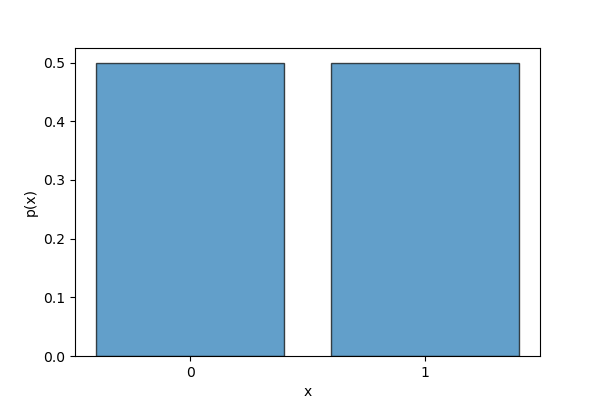
\includegraphics[width=0.7\textwidth]{figures/chapter2/bernoulli.png}
    \caption{Representation of the bernoulli distribution of a random variable $x$, given the total number of trials $n$ and the individual probability of success $p$.}
    \label{fig:bernoulli1}
\end{figure}

\textbf{Example 1: Coin Toss}\\

A fair coin toss is a Bernoulli trial with

\begin{equation}
p = P(\text{Heads}) = P(\text{Tails}) = 0.5.
\end{equation}

And we can model it as:
\begin{equation}
x = 
\begin{cases}
1 & \text{if Heads} \\
0 & \text{if Tails}
\end{cases}
\end{equation}

Bernoulli trials form the basis for more complex models such as the \textbf{Binomial distribution}, which models the number of successes in a fixed number of independent Bernoulli trials.

\newpage

\section{Probability distributions}
So far we have introduced the idea of random events, and the concept of probability as a number to quantify surprise. For our present chapter, we will try to model such stochastic events such that we can make predictions. For that purpose, we will model that probability we just defined to be a descriptive - even better, \textit{predictive} - quantity. Let's begin by saying that not all random phenomena are equal. Hence, a basic way to classify and separate random events, is according to how their probabilities are \textit{distributed}.

\subsection{Binomial distribution}
The simplest case of random event we will describe are the so-called \textit{binomial} events. Cases where we make a certain number of measurements $n$, each with two or more possible outcomes, and we want to know the number of successes. For instance, what would be the probability of measuring, or observing, 5 heads if I toss 10 coins? Or what would be the probability of obtaining 5 times a 6, out of a total of 100 dice rolls? In all these cases we will call $x$ the number of successes we want to observe, $n$ the total number of trials, and $p$ the probability of success in each individual trial. The binomial distribution models the number of successes in a fixed number of independent trials, each with the same probability of success. It was developed by Jacob Bernoulli in the 17th century while studying the probability of repeated Bernoulli trials. His work laid the foundation for the Law of Large Numbers.\\

Intuitively, this distribution is useful when considering repeated experiments with two possible outcomes (success or failure). For example, flipping a fair coin multiple times follows a binomial pattern. We will say that the probability of observing $x$ successes in $n$ total tries, given individual probability of success $p$, is given by:
\begin{equation}
    P(x; n, k) = \binom{n}{x} p^x (1-p)^{n-x},
\end{equation}
This is normally referred to as a probability \textit{mass} distribution. The reason for that, as we will discuss later, is to distinguish such events from other types of events called continuous, for which we will define \text{density} distributions. For now, just keep probability mass distribution as a fancy name, or probability distribution, for simplicity. Let's break this expression down in a couple of examples.

\begin{figure}[ht]
    \centering
    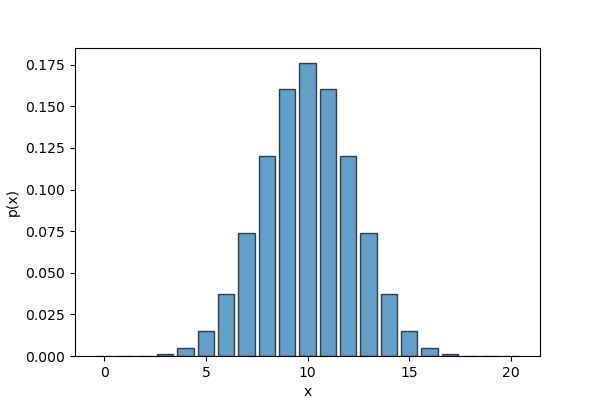
\includegraphics[width=0.7\textwidth]{figures/chapter2/binomial.png}
    \caption{Representation of the binomial distribution of a random variable $x$, given the total number of trials $n$ and the individual probability of success $p$.}
    \label{fig:binomial1}
\end{figure}

\textbf{Example 1:} Suppose we flip a fair coin 5 times ($n=5$) and want to find the probability of getting exactly 3 heads ($p=0.5$):
\begin{align}
    P\bigg(x=5; n = 10; p = \frac{1}{2}\bigg) = &\binom{5}{3} \bigg(\frac{1}{2}\bigg)^3 \bigg(1 - \frac{1}{2}\bigg)^2  \notag \\
    &\binom{5}{3} \bigg(\frac{1}{2}\bigg)^3 \bigg(1 - \frac{1}{2}\bigg)^2  \notag \times 0.25 = 0.3125.
\end{align}\\

\textbf{Example 2:} Suppose we flip a fair coin 5 times ($n=5$) and want to find the probability of getting exactly 3 heads ($p=0.5$):
\begin{equation}
    P\bigg(x=5; n = 10; p = \frac{1}{3}\bigg) = \binom{5}{3} \bigg(\frac{1}{2}\bigg)^3 \bigg(1 - \frac{1}{2}\bigg)^2 = 10 \times 0.125 \times 0.25 = 0.3125. \notag
\end{equation}\\

\textbf{Example 3:} Suppose we flip a fair coin 5 times ($n=5$) and want to find the probability of getting exactly 3 heads ($p=0.5$):
\begin{equation}
    P\bigg(x=5; n = 10; p = \frac{1}{6}\bigg) = \binom{5}{3} \bigg(\frac{1}{2}\bigg)^3 \bigg(1 - \frac{1}{2}\bigg)^2 = 10 \times 0.125 \times 0.25 = 0.3125. \notag
\end{equation}\\

\newpage
\subsection{Poisson distribution}
The next kind of random event we will discuss are the \textit{Poisson} distributed, named after the french mathematician Sim\'eon Denis Poisson, who tried to model to events that were random but with a known average rate, such as the number of people crossing a street per day, or the number of customers entering a store, or emails received per hour.
As a note, this distribution was introduced in quite recent times, in the early 19th century to model rare events. It is particularly useful for counting occurrences over a fixed interval of time or space. 

The probability mass function for observing a number of events $x$ if we know the average rate $\lambda$ is:
\begin{equation}
    P(x; \lambda) = \frac{\lambda^x e^{-\lambda}}{x!},
\end{equation}
Again, let's consider a couple of examples to illustrate Poisson distributed events.

\begin{figure}[ht]
    \centering
    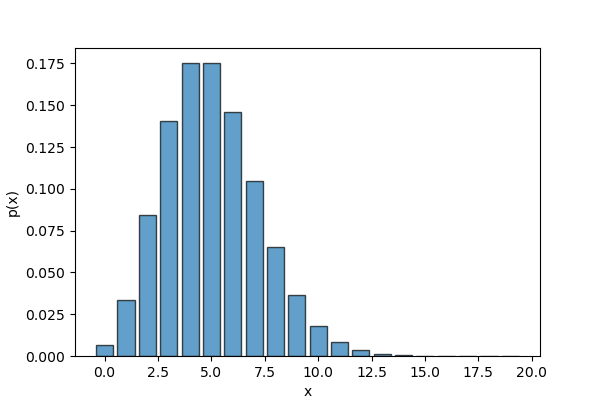
\includegraphics[width=0.7\textwidth]{figures/chapter2/poisson.png}
    \caption{Representation of the Poisson distribution of a random variable $x$, given the number of observations $\lambda$ as a parameter.}
    \label{fig:poisson1}
\end{figure}

\textbf{Example 1:} We would like to know the probability of observing exactly 5 cancer patients in a hospital over a week, if we know the average number ($\lambda = 3$) patients per week.
\begin{equation}
    P(x=5; \lambda = 3) = \frac{3^5 e^{-3}}{5!} = \frac{243 e^{-3}}{120} \approx 0.1008. \notag
\end{equation}\\

\textbf{Example 2:} Let's now ask a similar, but different question. So far, we have only focused on the probability of observing \textit{exactly} one particular outcome. But we could ask as well, what would be the probability observing 5 \textit{or less} cancer patients in that same hospital ($\lambda = 3$) patients per week.
\begin{align}
    P(x \leq 5; \lambda = 3) &= P(x=0; \lambda = 3) + P(x=1; \lambda = 3) + P(x=2; \lambda = 3) \notag \\
    &\quad + P(x=3; \lambda = 3) + P(x=4; \lambda = 3) + P(x=5; \lambda = 3) \notag
\end{align}\\

This sum of probabilities up to a given value is normally referred to as the \textit{cumulative probability}, \textit{cumulative distribution function}, or cdf.\\

\begin{figure}[ht]
    \centering
    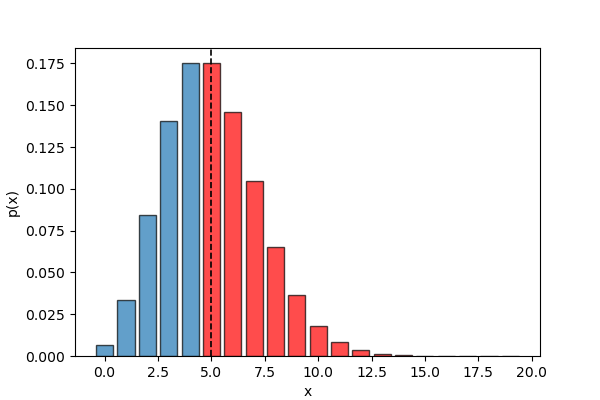
\includegraphics[width=0.7\textwidth]{figures/chapter2/poisson_highlight.png}
    \caption{Representation of the Poisson distribution of a random variable $x$, given the number of observations $\lambda$ as a parameter.}
    \label{fig:poisson2}
\end{figure}

\textbf{Example 3:} Now let's ask the opposite question. What would be the probability of observing \textit{at least} 5 patients in that same hospital?
\begin{align}
    P(x \leq 5; \lambda = 3) &= P(x=0; \lambda = 3) + P(x=1; \lambda = 3) + P(x=2; \lambda = 3) \notag \\
    &\quad + P(x=3; \lambda = 3) + P(x=4; \lambda = 3) + P(x=5; \lambda = 3) \notag
\end{align}\\

Given unitarity, we can just compute it as
\begin{equation}
    P(x > 5; \lambda = 3) = 1 - P(x \leq 5; \lambda = 3) = 1 - CDF(5; \lambda = 3). \notag
\end{equation}\\

\newpage
\subsection{Uniform distribution}
The last example of such discrete random - remember that by discrete we mean \textit{countable} number of outcomes -  will be those which are \textit{uniformly} distributed. That means that all possible outcomes are equally probable, such as rolling a fair die, or tossing a coin.

The uniform distribution represents a scenario where all outcomes in an interval $[a, b]$ are equally likely. This distribution has been used since antiquity, especially in early probability and gambling studies.

The probability of observing a particular result $x$ in a given range $[a, b]$ is:
\begin{equation}
    f(x; a, b) = \frac{1}{b-a}, \quad a \leq x \leq b.
\end{equation}

\begin{figure}[ht]
    \centering
    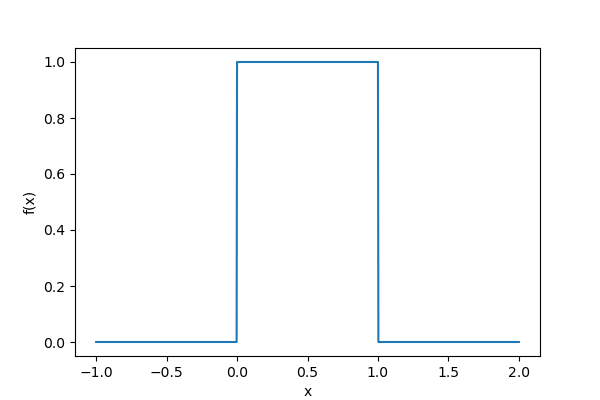
\includegraphics[width=0.7\textwidth]{figures/chapter2/uniform.png}
    \caption{Representation of the uniform distribution of a random variable $x$, given the boundary parameters $a$, $b$.}
    \label{fig:uniform1}
\end{figure}

\textbf{Example 1:} If a random number is chosen from the interval [2, 10], the probability density is:
\begin{equation}
    f(x; a, b) = \frac{1}{10-2} = 0.125.
\end{equation}

\textbf{Example 2:} If a random number is chosen from the interval [2, 10], the probability density is:
\begin{equation}
    f(x; a, b) = \frac{1}{10-2} = 0.125.
\end{equation}

\textbf{Example 3:} If a random number is chosen from the interval [2, 10], the probability density is:
\begin{equation}
    f(x; a, b) = \frac{1}{10-2} = 0.125.
\end{equation}

\newpage

So far we have focused on discrete events, that is, scenarios where the number of possible outcomes was an integer number. Now we will encounter a second family of stochastic processes, the ones we will refer to as continuous. In the discrete case, we were implicitly using the frequentist definition of probability, as a number that represents the ratio of how many times we will observe a particular result, if we endlessly repeat (...).\\

But let's try to face a different scenario. What would happen if we try to guess the probability of measuring something which does hace an infinite number of possible outcomes, spread on a continuous range? (e.g., the probability of measuring the height of a person an get 1.75 cm, or the temperature in a room and get 25 degrees, ...). Here we notice that, if we keep the definition of probability we used in the case of the Binomial, the Poisson, etc, we would get something like:

\begin{equation}
P(x = x_{0}) = \frac{\text{number of times I get $x_{0}$}}{\text{number of times I get any other result}}
\end{equation}

Note that now, the possible results are not just 1, 2, ..., n, but actually infinite more and spread over a continuous range. The outcome of measuring a temperature could be the $T = 25$ we want, but also $T = 24.999$ and $T = 25.001$, and there infinite other possible results between these two. No matter how precise our measurement devices, are, between any pair of results, we would have an infinite number of cases where we obtain a different result. Hence, applying the frequentist definition of probability would lead to:

\begin{equation}
P(x = x_{0}) = \frac{\text{number of times I get $x_{0}$}}{\text{number of times I get any other result}} = \frac{n}{\infty} = 0
\end{equation}

We would get that the probability of obtaining \textit{any result} would be exactly zero.\\

Let's pause for a moment and think about what happened. At the very beginning of this chapter we said that the quantity $P(x)$ was used to represent information - also certainty, surprise - and computed using the frequentist approach, meaning the \textit{ratio of favorable cases and total cases}. But that was assuming we had a finite set or possibilities, or measure space.

\begin{itemize}
\item Discrete (coins, dice, counting) $\longrightarrow$ finite, \textit{countable} outcomes
\item Continuous (temperature, energy, concentration, ...) $\longrightarrow$ infinite, \textit{uncountable}
\end{itemize}

For such cases we will define a mathematical quantity, similar to that we called probability, which represents analogous information, but considering the fact we are dealing with a continuous event. We will call it \textit{probability density} or \textit{density} for simplicity, and we will denote it with $f(x)$. Note that we can distinguish it from the probability in discrete events $P(x_{i})$, where we used the subscript $x_{i}$ to represent that the random variable could take just a finite set of values ($x_{1}$, $x{2}$, etc).

\begin{itemize}
\item Discrete (coins, dice, counting) $\longrightarrow$ Probability $P(x_{i})$ | $\sum_{i = 1}^{\infty} P(x_{i}) = 1$
\item Continuous (temperature, energy, concentration, ...) $\longrightarrow$ Probability density f(x) | $\int_{i = 0}^{\infty} f(x) dx = 1$
\end{itemize}

In the same way we imposed that probability needs to obey unitarity, we will impose that property in our recently defined probability density $f(x)$. The way we represent the sum for all possible cases in the continuous case, is just imposing that the integral of the function $f(x)$ is 1. This is just an example of \textit{normalization}, that we will explore further in chapter 4.

\newpage
\subsection{Gaussian distribution}
Introduced by Carl Friedrich Gauss, the normal distribution became central to statistics due to the Central Limit Theorem (CLT). It describes how averages of large samples tend to form a bell-shaped curve.

Intuitively, many natural and social phenomena follow a normal distribution, such as human heights and test scores.

Introduced by Carl Friedrich Gauss, the normal distribution became central to statistics due to the Central Limit Theorem (CLT). It describes how averages of large samples tend to form a bell-shaped curve.

Intuitively, many natural and social phenomena follow a normal distribution, such as human heights and test scores.

The probability density function is:
\begin{equation}
    f(x; \mu, \sigma) = \frac{1}{\sigma \sqrt{2\pi}} e^{-\frac{(x-\mu)^2}{2\sigma^2}}.
\end{equation}

\begin{figure}[ht]
    \centering
    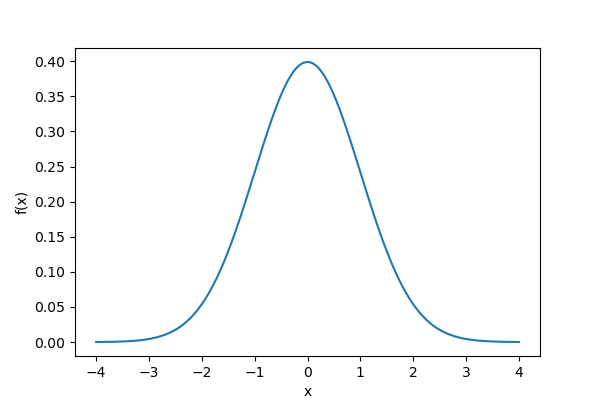
\includegraphics[width=0.7\textwidth]{figures/chapter2/normal.png}
    \caption{Representation of the gaussian distribution of a random variable $x$, given the mean value $\mu$ and standard deviation $\sigma$ parameters.}
    \label{fig:gaussian1}
\end{figure}

\textbf{Example 1:} If human heights are normally distributed with mean $\mu=170$ cm and standard deviation $\sigma=10$ cm, the probability density of someone being exactly 180 cm is:
\begin{equation}
    f(180) = \frac{1}{10 \sqrt{2\pi}} e^{-\frac{(180-170)^2}{2(10)^2}} \approx 0.0242.
\end{equation}

\textbf{Example 2:} If human heights are normally distributed with mean $\mu=170$ cm and standard deviation $\sigma=10$ cm, the probability density of someone being exactly 180 cm is:
\begin{equation}
    f(180) = \frac{1}{10 \sqrt{2\pi}} e^{-\frac{(180-170)^2}{2(10)^2}} \approx 0.0242.
\end{equation}

\textbf{Example 3:} If human heights are normally distributed with mean $\mu=170$ cm and standard deviation $\sigma=10$ cm, the probability density of someone being exactly 180 cm is:
\begin{equation}
    f(180) = \frac{1}{10 \sqrt{2\pi}} e^{-\frac{(180-170)^2}{2(10)^2}} \approx 0.0242.
\end{equation}

\newpage
\subsection{Exponential distribution}
The exponential distribution models waiting times between Poisson process events. It has been widely applied in reliability analysis and survival studies.

Intuitively, it describes situations where the probability of waiting a certain time between events remains constant, such as time between bus arrivals.

The exponential distribution models waiting times between Poisson process events. It has been widely applied in reliability analysis and survival studies.

Intuitively, it describes situations where the probability of waiting a certain time between events remains constant, such as time between bus arrivals.

The probability density function is:
\begin{equation}
    f(x; \lambda) = \lambda e^{-\lambda x}, \quad x \geq 0.
\end{equation}

\begin{figure}[ht]
    \centering
    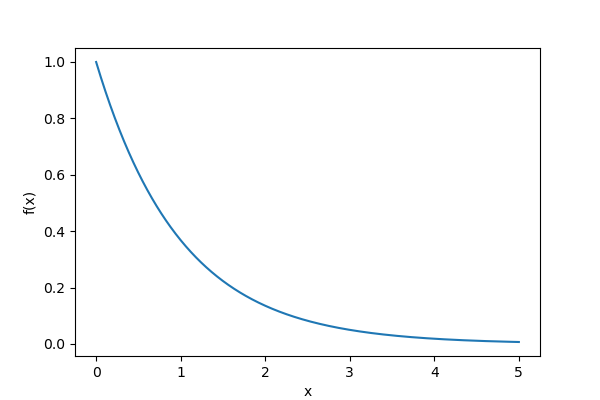
\includegraphics[width=0.7\textwidth]{figures/chapter2/exponential.png}
    \caption{Representation of the exponential distribution of a random variable $x$, given the decay rate $\lambda$.}
    \label{fig:exponential1}
\end{figure}

\textbf{Example 1:} If a call center receives calls at an average rate of $\lambda = 2$ per minute, the probability that the next call arrives after more than 2 minutes is:
\begin{equation}
    P(X > 2) = e^{-2(2)} = e^{-4} \approx 0.0183.
\end{equation}

\textbf{Example 2:} If a call center receives calls at an average rate of $\lambda = 2$ per minute, the probability that the next call arrives after more than 2 minutes is:
\begin{equation}
    P(X > 2) = e^{-2(2)} = e^{-4} \approx 0.0183.
\end{equation}

\textbf{Example 3:} If a call center receives calls at an average rate of $\lambda = 2$ per minute, the probability that the next call arrives after more than 2 minutes is:
\begin{equation}
    P(X > 2) = e^{-2(2)} = e^{-4} \approx 0.0183.
\end{equation}

% Chapter - Parameter estimation
\chapter{Parameter estimation}

\section{Prediction vs inference}
In the previous chapters we have introduced the mathematical theory of probability. That is, we have developed a series of tools, a \textit{theory}, which enables us to make predictions in stochastic processes. But, contrary to what is normally explain in introductory courses, science is not always headed in the theory and experiment direction. There can be cases, as we will soon see, where hypothesis are formulated for a given phenomena, and no prediction is made. In such cases, it is from measurement that we will try to see, or \textit{infer} if our hypothesis are compatible with given data. Indeed, most modern data analysis and hypothesis testing lie in the inferential statistics, rather than predictive probability.

The difference between prediction and inference has been a topic of interest in statistics and data science for centuries. While both concepts involve drawing conclusions from data, their goals, methodologies, and historical development differ significantly.\\

The roots of inference trace back to classical statistics, particularly the work of Pierre-Simon Laplace (1749–1827) and Carl Friedrich Gauss (1777–1855), who developed probability theory and the method of least squares. Their work laid the foundation for statistical inference, which aims to understand relationships between variables and make generalizable conclusions about populations from samples.\\

For example, Laplace used probability theory to estimate the population of France, introducing Bayesian inference, which provides a framework for updating beliefs based on observed data. Gauss contributed the normal distribution and least squares estimation, which became essential for making inferences about unknown parameters.\\

On the other hand, prediction as a primary goal gained traction much later, particularly in the 20th century with the rise of machine learning. The focus shifted from understanding relationships to optimizing models that generalize well to unseen data. In 2001, Leo Breiman, in his seminal paper "Statistical Modeling: The Two Cultures," highlighted the distinction, arguing that traditional statistics emphasized inference, whereas modern machine learning prioritized prediction.\\

Inference seeks to explain why and how variables relate. The key idea is causality and interpretability: given a dataset, inference aims to answer questions such as: Does smoking cause lung cancer, or is the correlation due to other confounding factors? How does an increase in temperature affect ice cream sales? What are the most significant predictors of house prices? Statistical techniques such as hypothesis testing, confidence intervals, and regression analysis help researchers understand these relationships. The emphasis is on estimating parameters and determining statistical significance rather than simply making accurate predictions. A classic example is Sir Ronald Fisher (1890–1962), who developed maximum likelihood estimation (MLE) to infer parameters of probability distributions. Fisher’s work allowed statisticians to estimate relationships between variables and quantify uncertainty.\\

Prediction focuses on accuracy and generalization rather than explaining causality. The goal is to create a model that performs well on new, unseen data, even if the underlying relationships between variables are not fully understood. For example, in modern deep learning, neural networks can recognize faces with high accuracy but offer little interpretability in how they make decisions. Unlike inference, which aims to understand why a pattern exists, prediction is about making the best possible guess given the available data. A key contributor to predictive modeling was Andrey Kolmogorov (1903–1987), who formalized probability theory and stochastic processes. His work laid the foundation for modern probabilistic models used in machine learning and artificial intelligence. Later, Vapnik and Chervonenkis (1971) developed statistical learning theory, which introduced VC dimension, a measure of a model’s ability to generalize. This work led to the development of Support Vector Machines (SVMs), a key predictive tool in machine learning.\\

While Breiman’s paper emphasized the divide between the two approaches, modern data science integrates both. In many cases, understanding causal relationships (inference) can improve predictive performance, and accurate prediction can guide further investigations into causality. For example, epidemiologists use inference to understand how diseases spread, but they also use predictive models to forecast outbreaks. In finance, analysts infer factors affecting stock prices while using machine learning to predict market trends. By combining both approaches, we gain a more comprehensive understanding of data, allowing for both insightful interpretations and powerful predictions.

\section{Parameter estimation}
Another key difference we will discuss now, and quite a subtle one from the mathematical perspective, is that one between a \textit{variable} and a \textit{parameter}. Consider the example of a binomial experiment, e.g. tossing coins and asking for the probability of measuring a specific number of heads. There, we would write it as 

\begin{equation}
    P(x; n, p) = \binom{n}{k} p^x (1-p)^{n-x},
\end{equation}
where $n$ is the number of trials and $p$ is the probability of success.

In our previous examples, we have treated just $x$ as our variable of interest, but we could think about P as a function of three independent variables. The number of times we want to observe heads, the total number of trials, and the probability of success for each toss. Normally, we will call \textit{parameters}, to all these variables we will freeze for the purpose of our calculations, and either consider them either known, or fit them from data (...).
 
 \newpage 
 
\section{The Law of Large Numbers}

\subsection*{Introduction}
The Law of Large Numbers (LLN) is one of the fundamental theorems of probability theory. It was first formulated by Jacob Bernoulli in the late 17th century and later refined by other mathematicians, including Pafnuty Chebyshev. Bernoulli's work aimed to formalize how relative frequencies of events stabilize as the number of trials increases, providing the foundation for statistical inference. LLN plays a crucial role in statistics, finance, and machine learning, ensuring that averages computed from large samples are reliable estimates of expected values.

\subsection{Definition}
The Law of Large Numbers states that as the sample size increases, the sample mean approaches the expected value. Formally, if $X_1, X_2, \dots, X_n$ are independent and identically distributed (i.i.d.) random variables with expected value $\mathbb{E}[X] = \mu$, then:
\begin{equation}
    \bar{X}_n = \frac{1}{n} \sum_{i=1}^{n} X_i \to \mu \quad \text{as } n \to \infty.
\end{equation}

Consider flipping a fair coin multiple times. The proportion of heads observed converges to 0.5 as the number of flips increases. This illustrates that the observed average stabilizes around the theoretical probability.

\subsection{Types of LLN}
\begin{itemize}
    \item \textbf{Weak Law of Large Numbers (WLLN)}: Convergence in probability, i.e., for any $\epsilon > 0$, 
    \begin{equation}
        P(|\bar{X}_n - \mu| \geq \epsilon) \to 0 \quad \text{as } n \to \infty.
    \end{equation}
    \item \textbf{Strong Law of Large Numbers (SLLN)}: Almost sure convergence, i.e.,
    \begin{equation}
        P\left( \lim_{n \to \infty} \bar{X}_n = \mu \right) = 1.
    \end{equation}
\end{itemize}

\begin{figure}[ht]
    \centering
    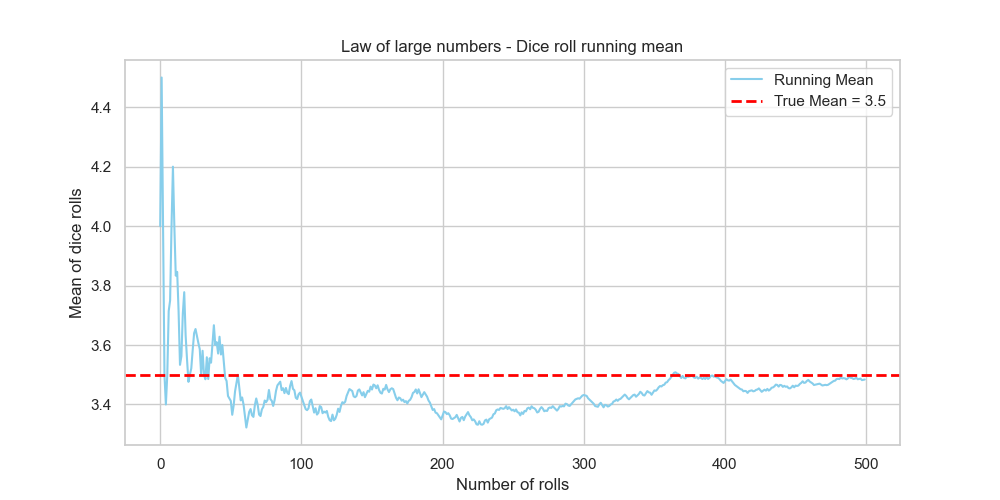
\includegraphics[width=0.7\textwidth]{figures/chapter3/law_large_numbers.png}
    \caption{Representation of the law or large numbers. The sample mean tends to the population mean as the number of rolls $n$ increases.}
    \label{fig:random}
\end{figure}

\textbf{Example:} Suppose we roll a fair six-sided die multiple times. The expected value of a roll is:
\begin{equation}
    \mathbb{E}[X] = \frac{1+2+3+4+5+6}{6} = 3.5.
\end{equation}
As we roll more dice, the sample mean of observed values gets closer to 3.5.

\newpage

\section{The Central Limit Theorem}

\subsection*{Introduction}
The Central Limit Theorem (CLT) was first discovered in the 18th century by Abraham de Moivre and later developed by Pierre-Simon Laplace and Carl Friedrich Gauss. It formalizes the idea that the distribution of sample means tends toward a normal distribution, regardless of the shape of the original population distribution. The CLT is fundamental in inferential statistics, allowing researchers to make predictions and construct confidence intervals for population parameters based on sample data.

\subsection{Definition}
The Central Limit Theorem states that for a large enough sample size, the sampling distribution of the sample mean follows a normal distribution, regardless of the original population distribution. Formally, if $X_1, X_2, \dots, X_n$ are i.i.d. random variables with mean $\mu$ and variance $\sigma^2$, then the standardized sample mean:
\begin{equation}
    Z = \frac{\bar{X}_n - \mu}{\sigma / \sqrt{n}}
\end{equation}
converges in distribution to a standard normal distribution $\mathcal{N}(0,1)$ as $n \to \infty$.

No matter the shape of the original distribution, when we take many samples and compute their means, the histogram of these sample means will resemble a normal curve as the sample size grows.

\begin{figure}[ht]
    \centering
    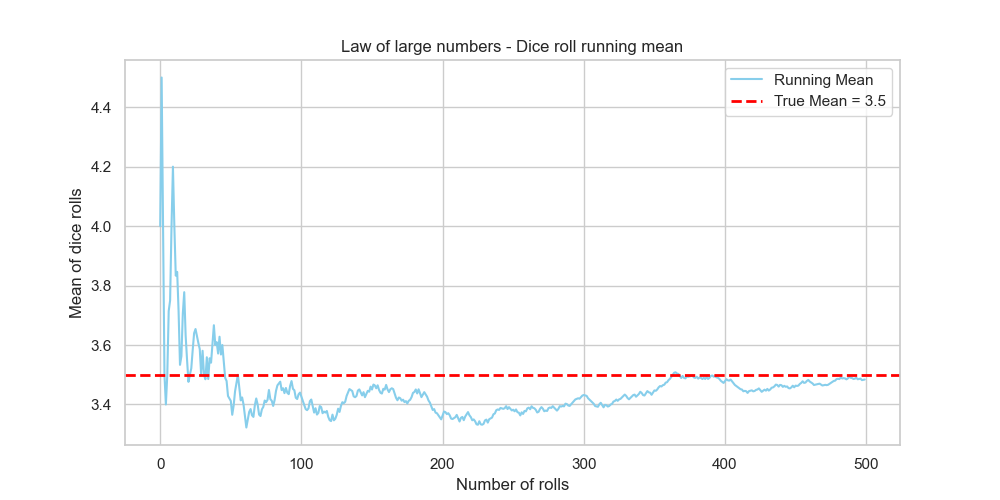
\includegraphics[width=0.7\textwidth]{figures/chapter3/law_large_numbers.png}
    \caption{Representation of the law or large numbers. The sample mean follows a gaussian distribution as the sample size $n$ increases.}
    \label{fig:random}
\end{figure}

\textbf{Example}: Consider rolling a fair six-sided die multiple times and computing the average outcome for groups of $n$ rolls. As $n$ increases, the distribution of these sample means approaches a normal distribution, centered at $\mu=3.5$.

\subsection{Applications}
\begin{itemize}
    \item Used in inferential statistics to approximate sampling distributions.
    \item Forms the basis for hypothesis testing and confidence intervals.
    \item Justifies the normality assumption in many statistical models.
\end{itemize}

% Chapter - Introduction to statistical inference
\chapter{Introduction to statistical inference}

\section{Prediction vs inference}
In the previous chapters we have introduced the mathematical theory of probability. That is, we have developed a series of tools, a \textit{theory}, which enables us to make predictions in stochastic processes. But, contrary to what is normally explain in introductory courses, science is not always headed in the theory and experiment direction. There can be cases, as we will soon see, where hypothesis are formulated for a given phenomena, and no prediction is made. In such cases, it is from measurement that we will try to see, or \textit{infer} if our hypothesis are compatible with given data. Indeed, most modern data analysis and hypothesis testing lie in the inferential statistics, rather than predictive probability.

\section{Hypothesis testing}
In the previous chapters we have introduced the mathematical theory of probability. That is, we have developed a series of tools, a \textit{theory}, which enables us to make predictions in stochastic processes. But, contrary to what is normally explain in introductory courses, science is not always headed in the theory and experiment direction. There can be cases, as we will soon see, where hypothesis are formulated for a given phenomena, and no prediction is made. In such cases, it is from measurement that we will try to see, or \textit{infer} if our hypothesis are compatible with given data. Indeed, most modern data analysis and hypothesis testing lie in the inferential statistics, rather than predictive probability.\\

So let's first ask ourselves the question. What is probability in the first place? What do we mean by it and what does it describe? Probability is nothing more, and nothing less, that a number we make up, a quantity we come up with, to quantify certainty. A number we will use to describe the amount of information we have about a random, or stochastic, event. For simplicity, we can make it range from 0 to 1, in the following way.

\newpage
\section{Statistic tests, p-values and significance}
Statistic tests, p-values and significance

\subsection{Compare sample mean with hypothesized value - One sample t-test}

Let's begin with the simplest example of hypothesis testing we can think of. The so-called \textit{one-sample t-test} is used to determine whether the mean of a single sample differs significantly from a known or hypothesized population mean. It assumes that the sample data are drawn from a normally distributed population. The test statistic is given by:
\[
    t = \frac{\bar{x} - \mu}{\sqrt{n}},
\]
where $\bar{x}$ is the sample mean, $\mu$ is the population mean, $s$ is the sample standard deviation, and $n$ is the sample size.

In the previous chapters we have introduced the mathematical theory of probability. That is, we have developed a series of tools, a \textit{theory}, which enables us to make predictions in stochastic processes. But, contrary to what is normally explain in introductory courses, science is not always headed in the theory and experiment direction. There can be cases, as we will soon see, where hypothesis are formulated for a given phenomena, and no prediction is made. In such cases, it is from measurement that we will try to see, or \textit{infer} if our hypothesis are compatible with given data. Indeed, most modern data analysis and hypothesis testing lie in the inferential statistics, rather than predictive probability.

\begin{figure}[ht]
    \centering
    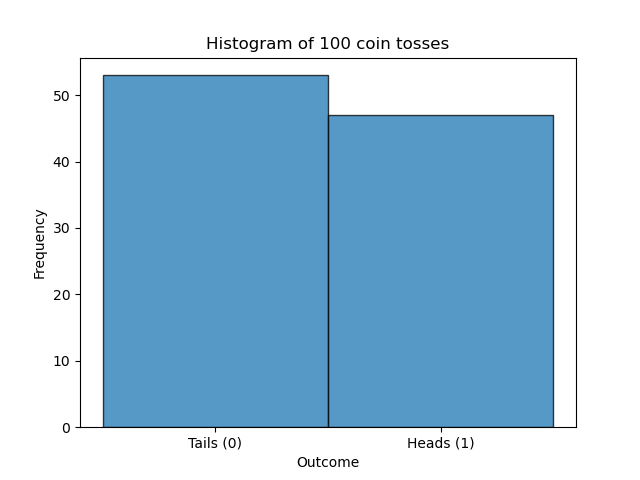
\includegraphics[width=0.7\textwidth]{figures/chapter4/t_1_sample_observations.png}
    \caption{Observations following gaussian distribution.}
    \label{fig:t_1_sample_obs}
\end{figure}

Inference seeks to explain why and how variables relate. The key idea is causality and interpretability: given a dataset, inference aims to answer questions such as: Does smoking cause lung cancer, or is the correlation due to other confounding factors? How does an increase in temperature affect ice cream sales? What are the most significant predictors of house prices? Statistical techniques such as hypothesis testing, confidence intervals, and regression analysis help researchers understand these relationships. The emphasis is on estimating parameters and determining statistical significance rather than simply making accurate predictions. A classic example is Sir Ronald Fisher (1890–1962), who developed maximum likelihood estimation (MLE) to infer parameters of probability distributions. Fisher’s work allowed statisticians to estimate relationships between variables and quantify uncertainty.\\

Prediction focuses on accuracy and generalization rather than explaining causality. The goal is to create a model that performs well on new, unseen data, even if the underlying relationships between variables are not fully understood. For example, in modern deep learning, neural networks can recognize faces with high accuracy but offer little interpretability in how they make decisions. Unlike inference, which aims to understand why a pattern exists, prediction is about making the best possible guess given the available data. A key contributor to predictive modeling was Andrey Kolmogorov (1903–1987), who formalized probability theory and stochastic processes. His work laid the foundation for modern probabilistic models used in machine learning and artificial intelligence. Later, Vapnik and Chervonenkis (1971) developed statistical learning theory, which introduced VC dimension, a measure of a model’s ability to generalize. This work led to the development of Support Vector Machines (SVMs), a key predictive tool in machine learning.\\

\begin{figure}[ht]
    \centering
    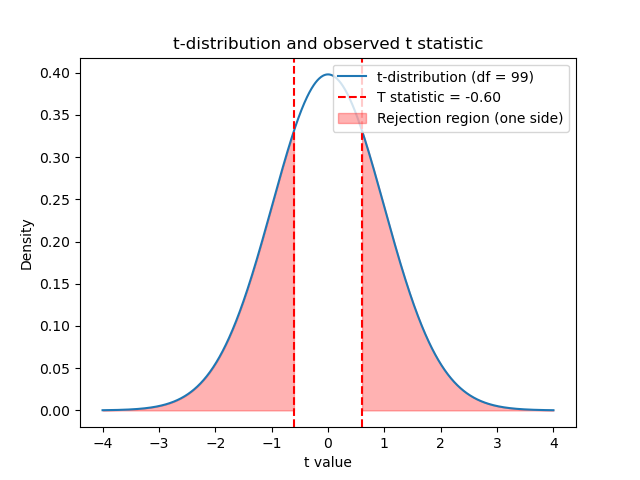
\includegraphics[width=0.7\textwidth]{figures/chapter4/t_1_sample_distribution.png}
    \caption{Representation of the Student's t distribution for given $t_{obs}$ value.}
    \label{fig:t_1_sample_dist}
\end{figure}

While Breiman’s paper emphasized the divide between the two approaches, modern data science integrates both. In many cases, understanding causal relationships (inference) can improve predictive performance, and accurate prediction can guide further investigations into causality. For example, epidemiologists use inference to understand how diseases spread, but they also use predictive models to forecast outbreaks. In finance, analysts infer factors affecting stock prices while using machine learning to predict market trends. By combining both approaches, we gain a more comprehensive understanding of data, allowing for both insightful interpretations and powerful predictions.

\newpage
\subsection{Compare sample means of two groups - Two sample t-test}

The next example we will encounter is an extension of the same question., The so-called \textit{two-sample t-test} is used to determine whether the sample means of two sets of observations are significantly different from one another. It assumes that the sample data are drawn from a normally distributed population. The test statistic is given by:
\[
    t = \frac{\bar{x_{1}} - \bar{x_{2}}}{\sqrt{\big(n_{1} - 1)^{2} + (n_{2} - 1)^{2}\big)}},
\]
where $\bar{x}$ is the sample mean, $\mu$ is the population mean, $s$ is the sample standard deviation, and $n$ is the sample size.

In the previous chapters we have introduced the mathematical theory of probability. That is, we have developed a series of tools, a \textit{theory}, which enables us to make predictions in stochastic processes. But, contrary to what is normally explain in introductory courses, science is not always headed in the theory and experiment direction. There can be cases, as we will soon see, where hypothesis are formulated for a given phenomena, and no prediction is made. In such cases, it is from measurement that we will try to see, or \textit{infer} if our hypothesis are compatible with given data. Indeed, most modern data analysis and hypothesis testing lie in the inferential statistics, rather than predictive probability.

\begin{figure}[ht]
    \centering
    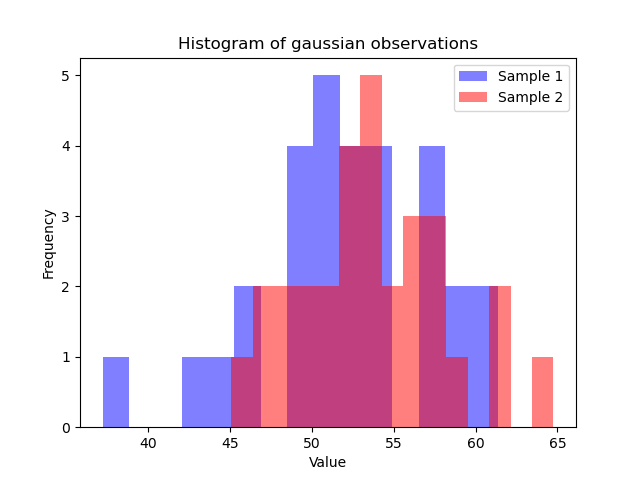
\includegraphics[width=0.7\textwidth]{figures/chapter4/t_2_samples_observations.png}
    \caption{Observations following gaussian distribution.}
    \label{fig:t_2_sample_obs}
\end{figure}

Inference seeks to explain why and how variables relate. The key idea is causality and interpretability: given a dataset, inference aims to answer questions such as: Does smoking cause lung cancer, or is the correlation due to other confounding factors? How does an increase in temperature affect ice cream sales? What are the most significant predictors of house prices? Statistical techniques such as hypothesis testing, confidence intervals, and regression analysis help researchers understand these relationships. The emphasis is on estimating parameters and determining statistical significance rather than simply making accurate predictions. A classic example is Sir Ronald Fisher (1890–1962), who developed maximum likelihood estimation (MLE) to infer parameters of probability distributions. Fisher’s work allowed statisticians to estimate relationships between variables and quantify uncertainty.\\

Prediction focuses on accuracy and generalization rather than explaining causality. The goal is to create a model that performs well on new, unseen data, even if the underlying relationships between variables are not fully understood. For example, in modern deep learning, neural networks can recognize faces with high accuracy but offer little interpretability in how they make decisions. Unlike inference, which aims to understand why a pattern exists, prediction is about making the best possible guess given the available data. A key contributor to predictive modeling was Andrey Kolmogorov (1903–1987), who formalized probability theory and stochastic processes. His work laid the foundation for modern probabilistic models used in machine learning and artificial intelligence. Later, Vapnik and Chervonenkis (1971) developed statistical learning theory, which introduced VC dimension, a measure of a model’s ability to generalize. This work led to the development of Support Vector Machines (SVMs), a key predictive tool in machine learning.\\

\begin{figure}[ht]
    \centering
    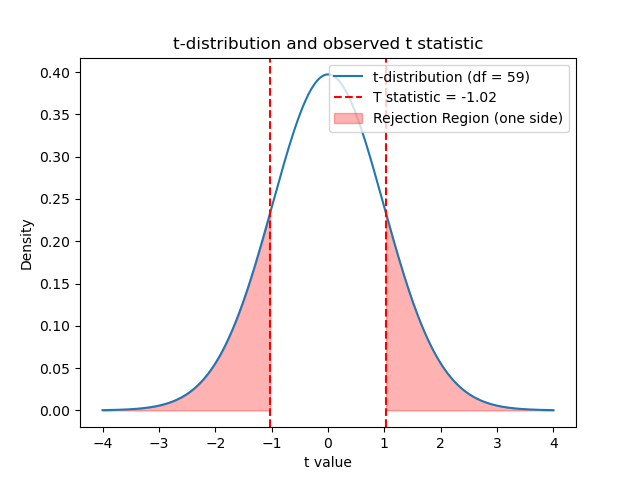
\includegraphics[width=0.7\textwidth]{figures/chapter4/t_2_samples_distribution.png}
    \caption{Representation of the Student's t distribution for given $t_{obs}$ value.}
    \label{fig:t_2_sample_obs}
\end{figure}

While Breiman’s paper emphasized the divide between the two approaches, modern data science integrates both. In many cases, understanding causal relationships (inference) can improve predictive performance, and accurate prediction can guide further investigations into causality. For example, epidemiologists use inference to understand how diseases spread, but they also use predictive models to forecast outbreaks. In finance, analysts infer factors affecting stock prices while using machine learning to predict market trends. By combining both approaches, we gain a more comprehensive understanding of data, allowing for both insightful interpretations and powerful predictions.

\newpage
\subsection{Compare sample variances of two groups - Fisher test}

The next example we will encounter is an extension of the same question., The so-called \textit{Fisher t-test}, or just $F$ test, is used to determine whether the sample variances of two sets of observations are significantly different from one another. It assumes that the sample data are drawn from a normally distributed population. The test statistic is given by:
\[
    f(x; d_{1}, d_{2}) = \frac{s_1}{s_2},
\]
where $\bar{x}$ is the sample mean, $\mu$ is the population mean, $s$ is the sample standard deviation, and $n$ is the sample size.

In the previous chapters we have introduced the mathematical theory of probability. That is, we have developed a series of tools, a \textit{theory}, which enables us to make predictions in stochastic processes. But, contrary to what is normally explain in introductory courses, science is not always headed in the theory and experiment direction. There can be cases, as we will soon see, where hypothesis are formulated for a given phenomena, and no prediction is made. In such cases, it is from measurement that we will try to see, or \textit{infer} if our hypothesis are compatible with given data. Indeed, most modern data analysis and hypothesis testing lie in the inferential statistics, rather than predictive probability.

\begin{figure}[ht]
    \centering
    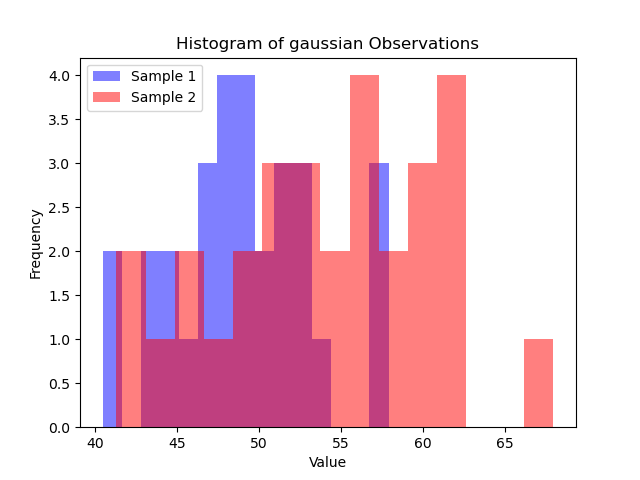
\includegraphics[width=0.7\textwidth]{figures/chapter4/f_observations.png}
    \caption{Observations following gaussian distribution.}
    \label{fig:f_obs}
\end{figure}

Inference seeks to explain why and how variables relate. The key idea is causality and interpretability: given a dataset, inference aims to answer questions such as: Does smoking cause lung cancer, or is the correlation due to other confounding factors? How does an increase in temperature affect ice cream sales? What are the most significant predictors of house prices? Statistical techniques such as hypothesis testing, confidence intervals, and regression analysis help researchers understand these relationships. The emphasis is on estimating parameters and determining statistical significance rather than simply making accurate predictions. A classic example is Sir Ronald Fisher (1890–1962), who developed maximum likelihood estimation (MLE) to infer parameters of probability distributions. Fisher’s work allowed statisticians to estimate relationships between variables and quantify uncertainty.\\

Prediction focuses on accuracy and generalization rather than explaining causality. The goal is to create a model that performs well on new, unseen data, even if the underlying relationships between variables are not fully understood. For example, in modern deep learning, neural networks can recognize faces with high accuracy but offer little interpretability in how they make decisions. Unlike inference, which aims to understand why a pattern exists, prediction is about making the best possible guess given the available data. A key contributor to predictive modeling was Andrey Kolmogorov (1903–1987), who formalized probability theory and stochastic processes. His work laid the foundation for modern probabilistic models used in machine learning and artificial intelligence. Later, Vapnik and Chervonenkis (1971) developed statistical learning theory, which introduced VC dimension, a measure of a model’s ability to generalize. This work led to the development of Support Vector Machines (SVMs), a key predictive tool in machine learning.\\

\begin{figure}[ht]
    \centering
    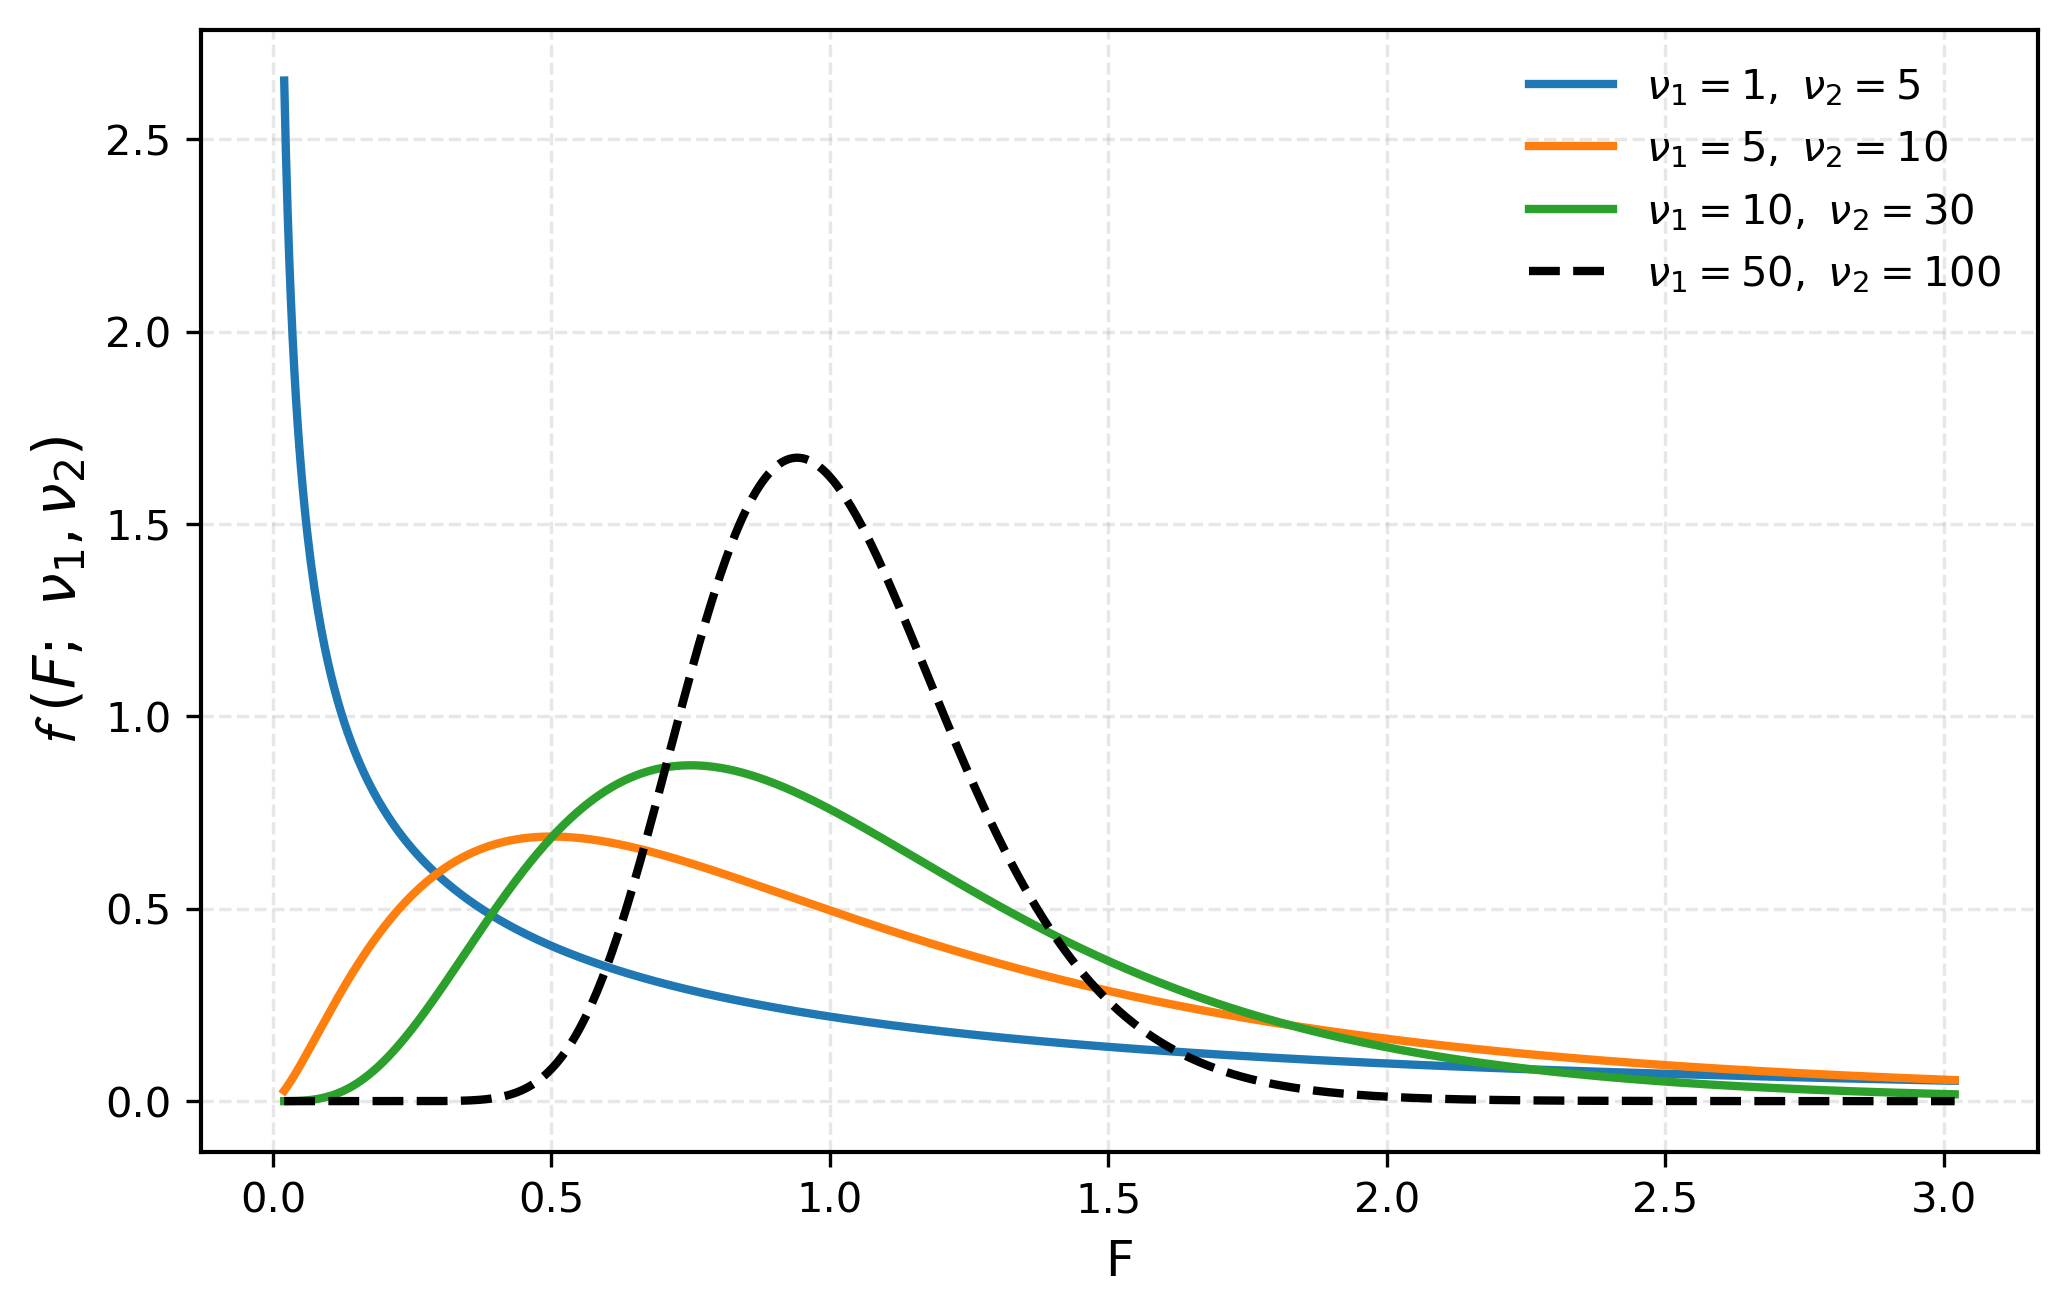
\includegraphics[width=0.7\textwidth]{figures/chapter4/f_distribution.png}
    \caption{Representation of the Fisher distribution for given $F_{obs}$ value.}
    \label{fig:f_dist}
\end{figure}

While Breiman’s paper emphasized the divide between the two approaches, modern data science integrates both. In many cases, understanding causal relationships (inference) can improve predictive performance, and accurate prediction can guide further investigations into causality. For example, epidemiologists use inference to understand how diseases spread, but they also use predictive models to forecast outbreaks. In finance, analysts infer factors affecting stock prices while using machine learning to predict market trends. By combining both approaches, we gain a more comprehensive understanding of data, allowing for both insightful interpretations and powerful predictions.

\newpage
\subsection{Compare more than two groups - ANOVA}

The next example we will encounter is an extension of the same question., The so-called \textit{Fisher t-test}, or just $F$ test, is used to determine whether the sample variances of two sets of observations are significantly different from one another. It assumes that the sample data are drawn from a normally distributed population. The test statistic is given by:
\[
    f(x; d_{1}, d_{2}) = \frac{s_1}{s_2},
\]
where $\bar{x}$ is the sample mean, $\mu$ is the population mean, $s$ is the sample standard deviation, and $n$ is the sample size.

In the previous chapters we have introduced the mathematical theory of probability. That is, we have developed a series of tools, a \textit{theory}, which enables us to make predictions in stochastic processes. But, contrary to what is normally explain in introductory courses, science is not always headed in the theory and experiment direction. There can be cases, as we will soon see, where hypothesis are formulated for a given phenomena, and no prediction is made. In such cases, it is from measurement that we will try to see, or \textit{infer} if our hypothesis are compatible with given data. Indeed, most modern data analysis and hypothesis testing lie in the inferential statistics, rather than predictive probability.

\begin{figure}[ht]
    \centering
    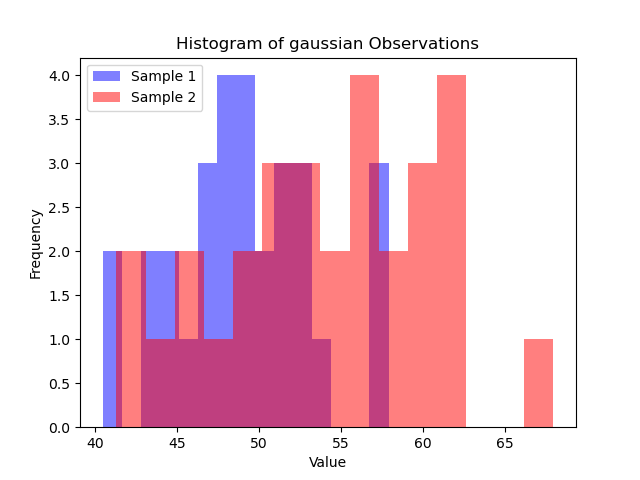
\includegraphics[width=0.7\textwidth]{figures/chapter4/f_observations.png}
    \caption{Observations following gaussian distribution.}
    \label{fig:f_obs}
\end{figure}

Inference seeks to explain why and how variables relate. The key idea is causality and interpretability: given a dataset, inference aims to answer questions such as: Does smoking cause lung cancer, or is the correlation due to other confounding factors? How does an increase in temperature affect ice cream sales? What are the most significant predictors of house prices? Statistical techniques such as hypothesis testing, confidence intervals, and regression analysis help researchers understand these relationships. The emphasis is on estimating parameters and determining statistical significance rather than simply making accurate predictions. A classic example is Sir Ronald Fisher (1890–1962), who developed maximum likelihood estimation (MLE) to infer parameters of probability distributions. Fisher’s work allowed statisticians to estimate relationships between variables and quantify uncertainty.\\

Prediction focuses on accuracy and generalization rather than explaining causality. The goal is to create a model that performs well on new, unseen data, even if the underlying relationships between variables are not fully understood. For example, in modern deep learning, neural networks can recognize faces with high accuracy but offer little interpretability in how they make decisions. Unlike inference, which aims to understand why a pattern exists, prediction is about making the best possible guess given the available data. A key contributor to predictive modeling was Andrey Kolmogorov (1903–1987), who formalized probability theory and stochastic processes. His work laid the foundation for modern probabilistic models used in machine learning and artificial intelligence. Later, Vapnik and Chervonenkis (1971) developed statistical learning theory, which introduced VC dimension, a measure of a model’s ability to generalize. This work led to the development of Support Vector Machines (SVMs), a key predictive tool in machine learning.\\

\begin{figure}[ht]
    \centering
    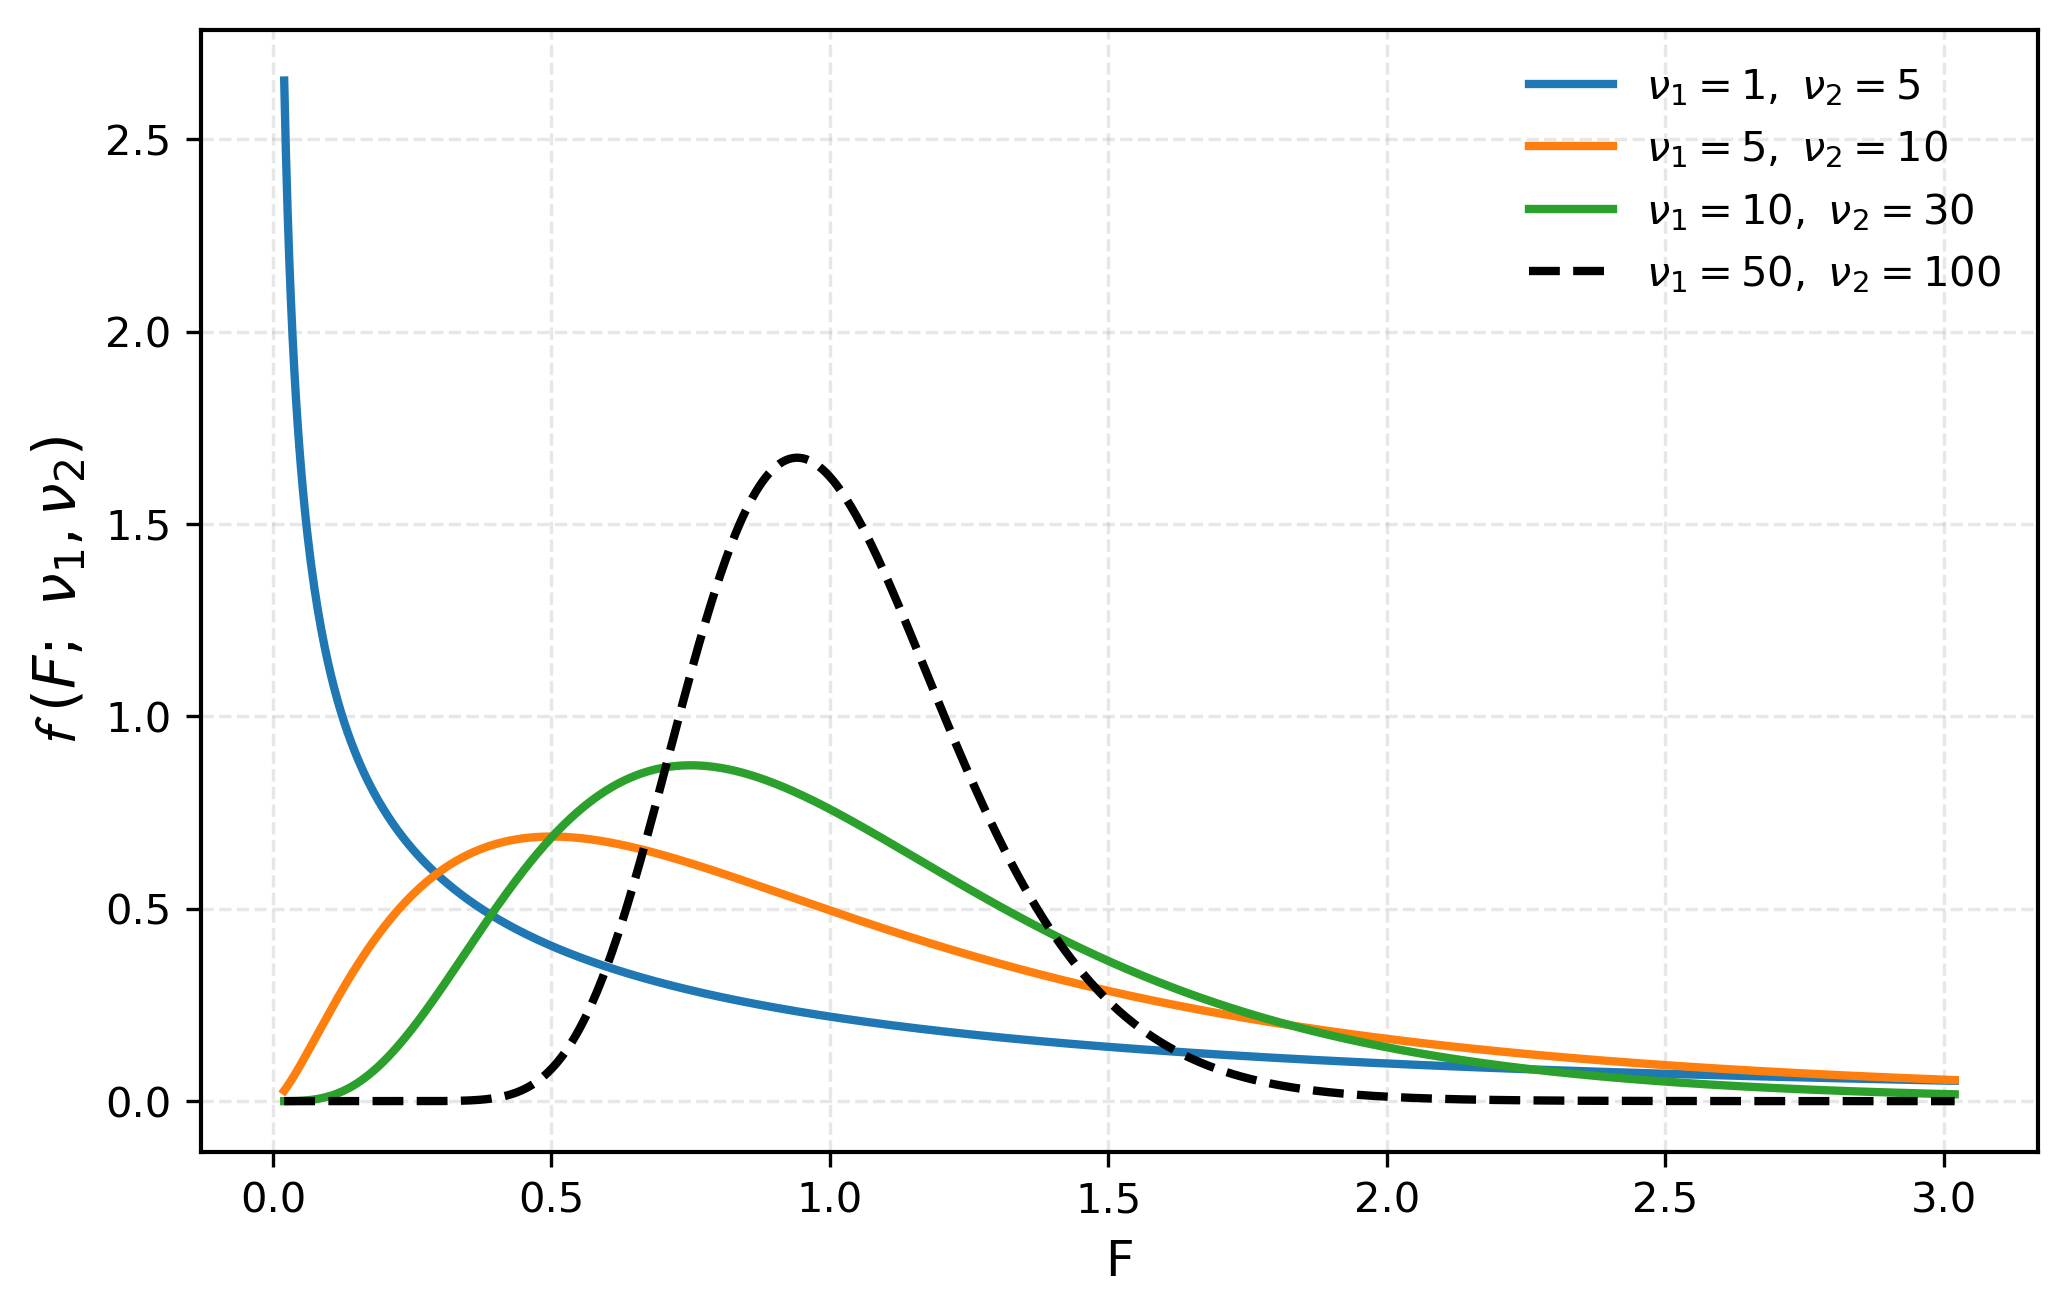
\includegraphics[width=0.7\textwidth]{figures/chapter4/f_distribution.png}
    \caption{Representation of the Fisher distribution for given $F_{obs}$ value.}
    \label{fig:f_dist}
\end{figure}

While Breiman’s paper emphasized the divide between the two approaches, modern data science integrates both. In many cases, understanding causal relationships (inference) can improve predictive performance, and accurate prediction can guide further investigations into causality. For example, epidemiologists use inference to understand how diseases spread, but they also use predictive models to forecast outbreaks. In finance, analysts infer factors affecting stock prices while using machine learning to predict market trends. By combining both approaches, we gain a more comprehensive understanding of data, allowing for both insightful interpretations and powerful predictions.

\newpage
\subsection{Compare distributions - $\chi^{2}$ test}

The next example we will encounter is an extension of the same question., The so-called \textit{Fisher t-test}, or just $F$ test, is used to determine whether the sample variances of two sets of observations are significantly different from one another. It assumes that the sample data are drawn from a normally distributed population. The test statistic is given by:
\[
    f(x; d_{1}, d_{2}) = \frac{s_1}{s_2},
\]
where $\bar{x}$ is the sample mean, $\mu$ is the population mean, $s$ is the sample standard deviation, and $n$ is the sample size.

In the previous chapters we have introduced the mathematical theory of probability. That is, we have developed a series of tools, a \textit{theory}, which enables us to make predictions in stochastic processes. But, contrary to what is normally explain in introductory courses, science is not always headed in the theory and experiment direction. There can be cases, as we will soon see, where hypothesis are formulated for a given phenomena, and no prediction is made. In such cases, it is from measurement that we will try to see, or \textit{infer} if our hypothesis are compatible with given data. Indeed, most modern data analysis and hypothesis testing lie in the inferential statistics, rather than predictive probability.

\begin{figure}[ht]
    \centering
    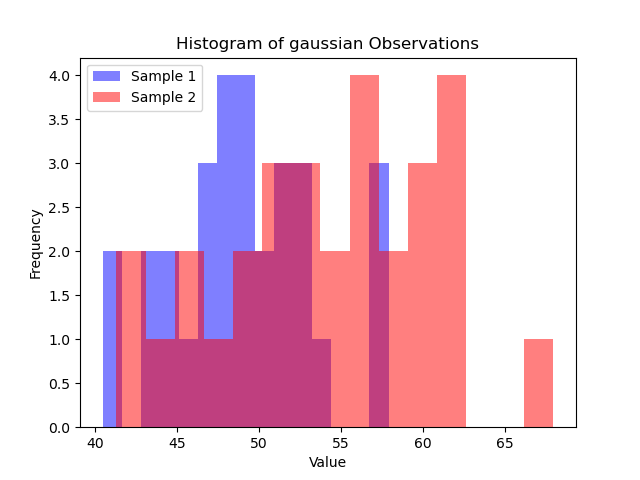
\includegraphics[width=0.7\textwidth]{figures/chapter4/f_observations.png}
    \caption{Observations following gaussian distribution.}
    \label{fig:f_obs}
\end{figure}

Inference seeks to explain why and how variables relate. The key idea is causality and interpretability: given a dataset, inference aims to answer questions such as: Does smoking cause lung cancer, or is the correlation due to other confounding factors? How does an increase in temperature affect ice cream sales? What are the most significant predictors of house prices? Statistical techniques such as hypothesis testing, confidence intervals, and regression analysis help researchers understand these relationships. The emphasis is on estimating parameters and determining statistical significance rather than simply making accurate predictions. A classic example is Sir Ronald Fisher (1890–1962), who developed maximum likelihood estimation (MLE) to infer parameters of probability distributions. Fisher’s work allowed statisticians to estimate relationships between variables and quantify uncertainty.\\

Prediction focuses on accuracy and generalization rather than explaining causality. The goal is to create a model that performs well on new, unseen data, even if the underlying relationships between variables are not fully understood. For example, in modern deep learning, neural networks can recognize faces with high accuracy but offer little interpretability in how they make decisions. Unlike inference, which aims to understand why a pattern exists, prediction is about making the best possible guess given the available data. A key contributor to predictive modeling was Andrey Kolmogorov (1903–1987), who formalized probability theory and stochastic processes. His work laid the foundation for modern probabilistic models used in machine learning and artificial intelligence. Later, Vapnik and Chervonenkis (1971) developed statistical learning theory, which introduced VC dimension, a measure of a model’s ability to generalize. This work led to the development of Support Vector Machines (SVMs), a key predictive tool in machine learning.\\

\begin{figure}[ht]
    \centering
    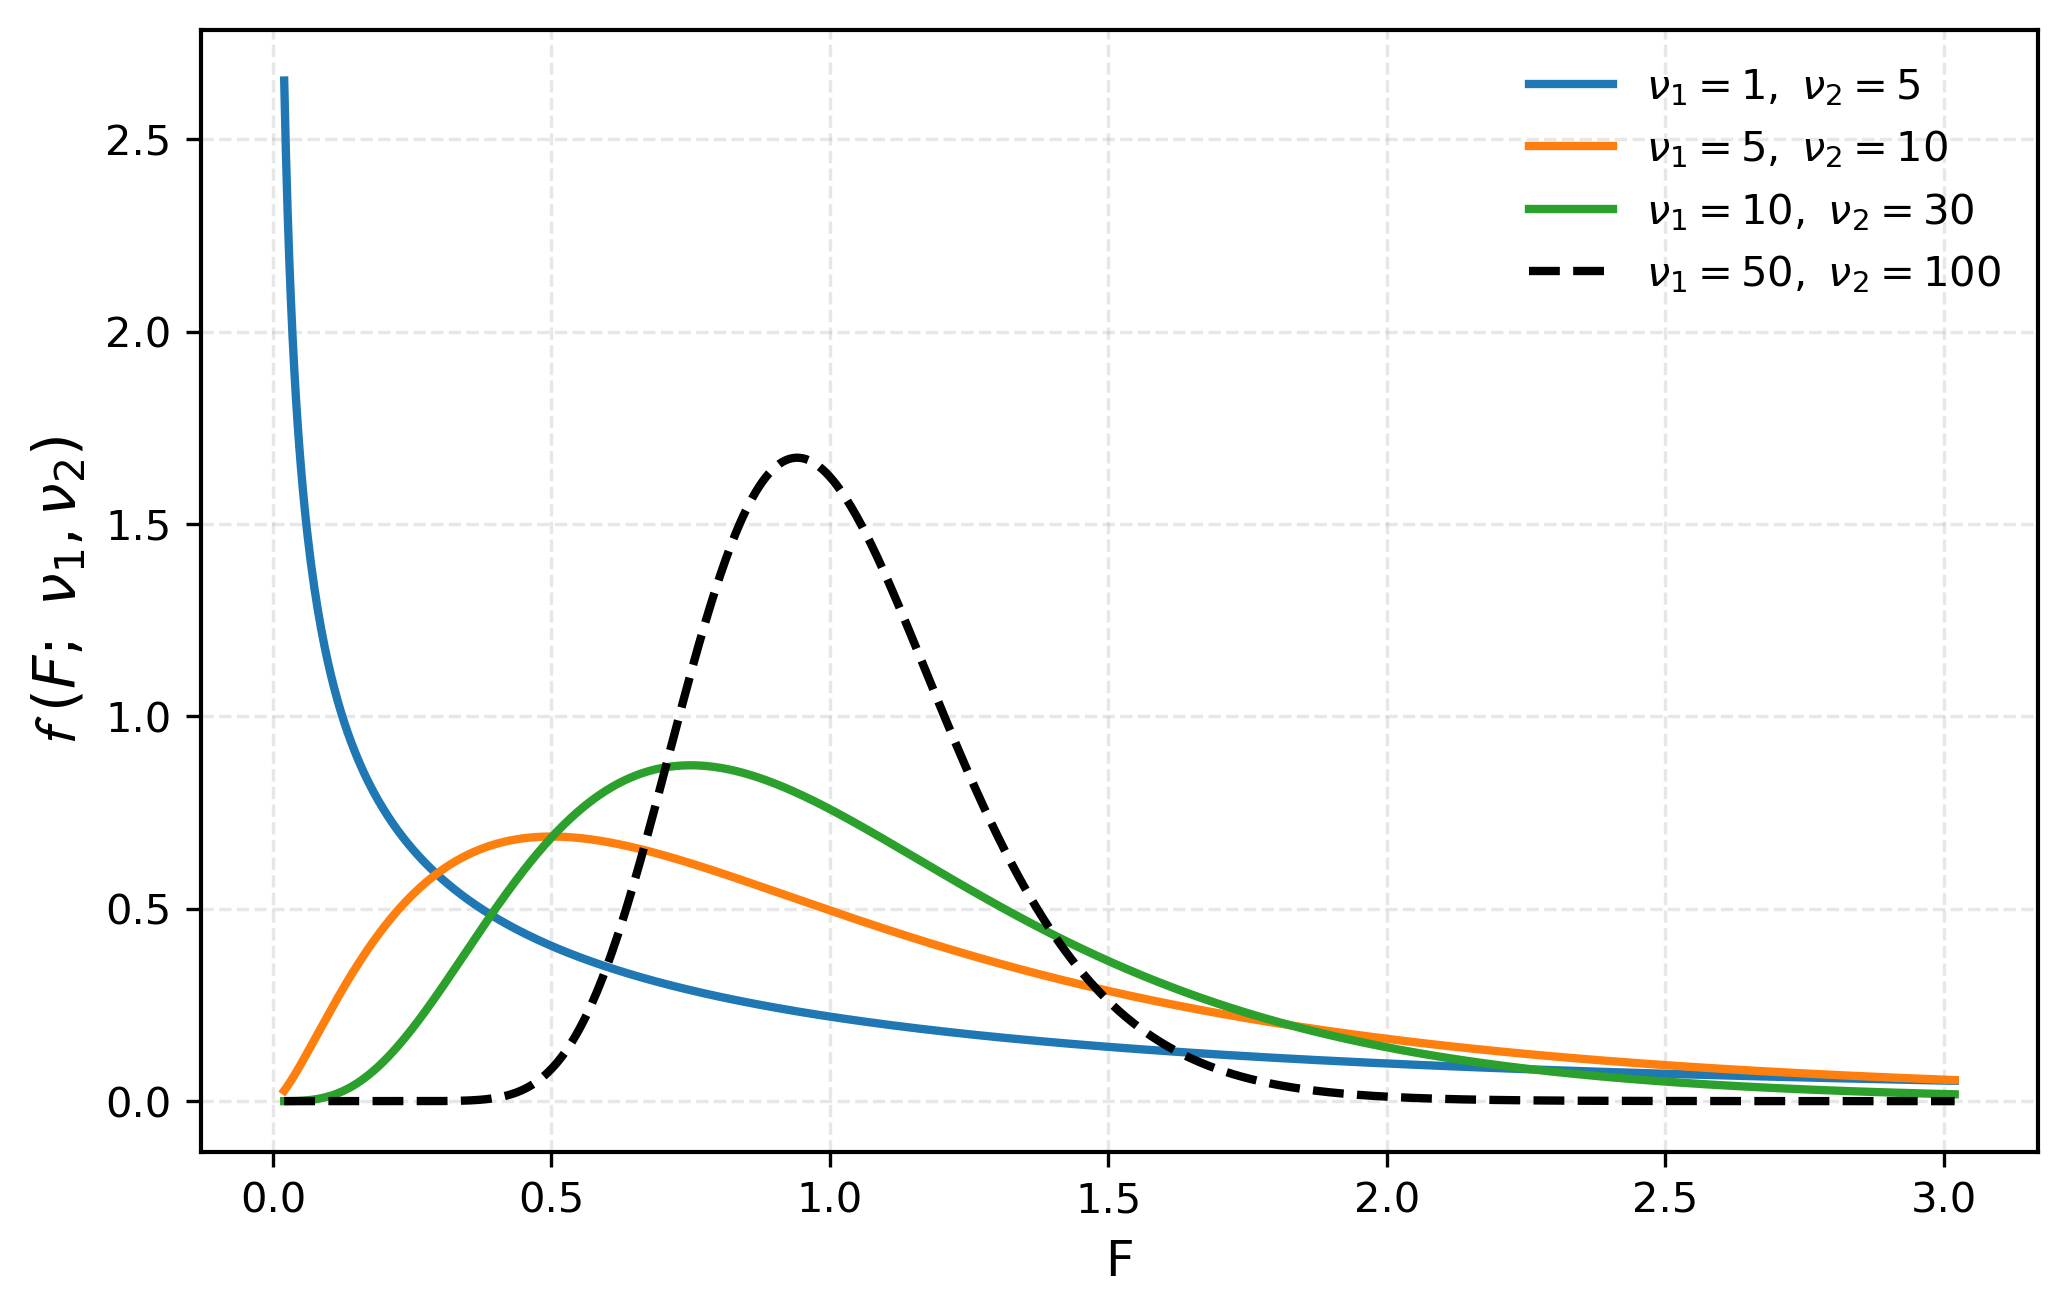
\includegraphics[width=0.7\textwidth]{figures/chapter4/f_distribution.png}
    \caption{Representation of the Fisher distribution for given $F_{obs}$ value.}
    \label{fig:f_dist}
\end{figure}

While Breiman’s paper emphasized the divide between the two approaches, modern data science integrates both. In many cases, understanding causal relationships (inference) can improve predictive performance, and accurate prediction can guide further investigations into causality. For example, epidemiologists use inference to understand how diseases spread, but they also use predictive models to forecast outbreaks. In finance, analysts infer factors affecting stock prices while using machine learning to predict market trends. By combining both approaches, we gain a more comprehensive understanding of data, allowing for both insightful interpretations and powerful predictions.

\newpage
\section{Parametric and non-parametric}

In the previous chapters we have introduced the mathematical theory of probability. That is, we have developed a series of tools, a \textit{theory}, which enables us to make predictions in stochastic processes. But, contrary to what is normally explain in introductory courses, science is not always headed in the theory and experiment direction. There can be cases, as we will soon see, where hypothesis are formulated for a given phenomena, and no prediction is made. In such cases, it is from measurement that we will try to see, or \textit{infer} if our hypothesis are compatible with given data. Indeed, most modern data analysis and hypothesis testing lie in the inferential statistics, rather than predictive probability.

Inference seeks to explain why and how variables relate. The key idea is causality and interpretability: given a dataset, inference aims to answer questions such as: Does smoking cause lung cancer, or is the correlation due to other confounding factors? How does an increase in temperature affect ice cream sales? What are the most significant predictors of house prices? Statistical techniques such as hypothesis testing, confidence intervals, and regression analysis help researchers understand these relationships. The emphasis is on estimating parameters and determining statistical significance rather than simply making accurate predictions. A classic example is Sir Ronald Fisher (1890–1962), who developed maximum likelihood estimation (MLE) to infer parameters of probability distributions. Fisher’s work allowed statisticians to estimate relationships between variables and quantify uncertainty.\\

Prediction focuses on accuracy and generalization rather than explaining causality. The goal is to create a model that performs well on new, unseen data, even if the underlying relationships between variables are not fully understood. For example, in modern deep learning, neural networks can recognize faces with high accuracy but offer little interpretability in how they make decisions. Unlike inference, which aims to understand why a pattern exists, prediction is about making the best possible guess given the available data. A key contributor to predictive modeling was Andrey Kolmogorov (1903–1987), who formalized probability theory and stochastic processes. His work laid the foundation for modern probabilistic models used in machine learning and artificial intelligence. Later, Vapnik and Chervonenkis (1971) developed statistical learning theory, which introduced VC dimension, a measure of a model’s ability to generalize. This work led to the development of Support Vector Machines (SVMs), a key predictive tool in machine learning.\\

While Breiman’s paper emphasized the divide between the two approaches, modern data science integrates both. In many cases, understanding causal relationships (inference) can improve predictive performance, and accurate prediction can guide further investigations into causality. For example, epidemiologists use inference to understand how diseases spread, but they also use predictive models to forecast outbreaks. In finance, analysts infer factors affecting stock prices while using machine learning to predict market trends. By combining both approaches, we gain a more comprehensive understanding of data, allowing for both insightful interpretations and powerful predictions.

\newpage
\section{Comparing data and normalization}
Comparing data and normalization

% Chapter - Introduction to bayesian statistics
\chapter{Introduction to bayesian statistics}

\section{The Bayes' theorem}
The Bayes' theorem.

\section{Bayesian vs frequentist}
Bayesian vs frequentist.

\section{Bayesian statistics}
Bayesian statistics.


% Chapter - Stochasticity and Markov processes
\chapter{Stochasticity and Markov processes}

\section{Stochasticity and Markov processes}

\section{Markov chains and hidden Markov models}

\section{Modern applications}


\backmatter
 
\begin{thebibliography}{999}

\bibitem{spiegelhalter2019art} 
David Spiegelhalter. 
\textit{The Art of Statistics: How to Learn from Data}. 
Basic Books, 2019.

\bibitem{degroot2012probability}
Morris H. DeGroot and Mark J. Schervish.
\textit{Probability and Statistics} (4th ed.).
Pearson, 2012.

\bibitem{mcfadden2011philosophy}
J. A. F. McFadden.
\textit{The Philosophy of Statistics}.
Wiley-Blackwell, 2011.

\end{thebibliography}

\end{document}
